\section{SURF}
SURF\footnote{SpeededUp Robust Features},introduceret af Herbert Bay et. al \cite{SURF} i 2006 er, ligesom SIFT, en samlet metode, bestående af en detektor og en deskriptor, der finder og beskriver blobs af forskellige størrelser. I forhold til SIFT, har SURF den fordel, at den beregningsmæssigt kan optimeres til at være hurtigere end SIFT, og metoden er mindre kompleks, da den består af færre beregningsskridt.
\subsection{Determinant of Hessian}
Determinant of Hessian eller \textit{DoH}: $\textbf{det}\mathcal{H}L$ , udgør feature detektoren i
SURF. DoH er baseret på Hessian matricen, som udregnes for hvert punkt $p=(x,y)$ i et billede:
\begin{equation}
\mathcal{H}(p, \sigma) = 
 \begin{bmatrix}
 	L_{xx}(p, \sigma) & L_{xy}(p, \sigma) \\
 	L_{xy}(p, \sigma) & L_{yy}(p, \sigma) 
 \end{bmatrix}
 \label{hessianmatrix}
\end{equation}
hvor $\sigma$ svarer til skalaen og $L_{xy} $, $L_{yy}$ og $L_{xx}$\eqref{lxx}, er den Gaussiske funktionen, partielt differentieret ifht. $xy$, $yy$ og $xx$.
\begin{equation}
L_{xx}(x, \sigma) = (\frac{\partial^2 }{\partial x^2 } G(x,y,\sigma)) * I
\label{lxx}
\end{equation}
Bay et.al anvender approkismerede, vægtede box filtrer $D_{xx}$, $D_{yy}$ og $D_{xy}$, der ved brug af integralbilleder nedsætter antallet af beregninger drastisk. Disse filtrer består udelukkende af værdier af -2,-1,0 eller 1. I implementeringen er disse boxfiltrer ikke anvendt, og er derved udregnet som i \eqref{lxx}, figur \ref{fig:lxxlyylxy} viser en illustration af de anvendte filtre.
\begin{figure}[H]
    \centering
    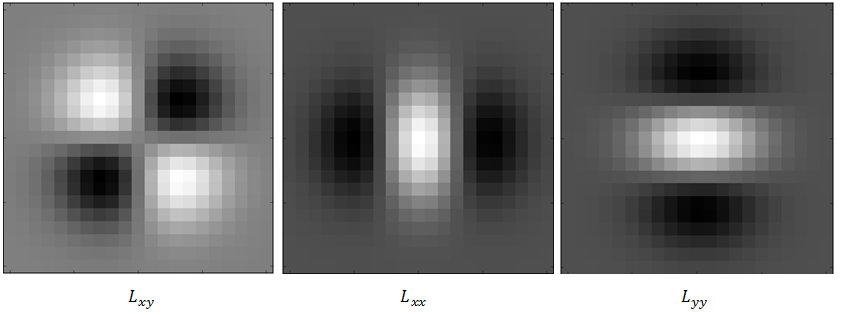
\includegraphics[width=0.75\textwidth]{fig/31.png}
     \vspace{-0.5em}
    \begin{center}    
       \caption{\textcolor{gray}{\footnotesize \textit{ }}}
    \label{fig:lxxlyylxy}
     \end{center}
     \vspace{-2.5em}
  \end{figure} \noindent
I metoden oprettes skalarummet ved iterativt at forøge størrelsen af filtrene, med $\sigma=1.2$, fremfor at forøge størrelsen af $\sigma$. For hver oktav, eksisterer, i denne implementering, fire billeder, foldet med fire forskellige filterstørrelser. For hver oktav, bruges nr. to filterstørrelse, fra forrige oktav til starten af den næste oktav, og størrelsen imellem filtre, fordobles fra forrige oktav, som vist i tabel \ref{fig:secderivfiltersize}. Her skal det bemærkes, at de andenafledte filtre, skal have dobbelt størrelse, af de førsteafledte, som er vist i tabel \ref{fig:firstderivfiltersize}
\begin{figure}[H]
    \centering
    \begin{center}    
    \begin{tabular}{ | l | l | l | l | l |}
    \hline
    oktav & filter str 1 & filter str 2 & filter str 3 & filter str 4 \\ \hline
    1 & 9 & 15 & 21 & 27 \\ \hline
  	2 & 15 & 27 & 39 & 51 \\ \hline
  	3 & 27 & 51 & 75 & 99 \\ \hline
  	4 & 51 & 99 & 147 & 195 \\ \hline
    \end{tabular}       
    \caption{\textcolor{gray}{\footnotesize \textit{Fire forskellige oktaver, og filterstørrelse, for et andenafledt filter}}}
    \label{fig:secderivfiltersize}
     \end{center}
     \vspace{-2.5em}
  \end{figure} \noindent
For hvert punkt i billederne opstilles Hessian matricen, hvorefter determinten udregnes for alle punkter i billederne. Bay et.al. udregner determinanten ved:
\begin{equation}
\textbf{det}\mathcal{H}_{approksimeret} = D_{xx}D_{yy}-wD_{xy}^2
\label{deerminantofhessian}
\end{equation}
, hvor $w$ er en vægt, tilføjet, for at balancere de approksimerede filtre og boks filtrene. Da denne implementering ikke anvender boks filtrer udregnes determinanten som:
\begin{equation}
\textbf{det}\mathcal{H} = L_{xx}L_{yy}-L_{xy}^2
\label{deerminantofhessian}
\end{equation}
Determinant of Hessian reagere på mørke og lyse blobs, ved positive svar. Derfor udvælges et lokalt maxima af et $3\times3\times3$ område af determinantbillederne, som vist på figur \ref{fig:difference}. Dette udføres for alle oktaver. Herefter udvælges korrekt subpixel placering, hvilket er en metode introduceret af David Lowe, også beskrevet i SIFT. Igen udføres dette skridt ved at fjerne punkter ikke lokaliseret tæt nok på ekstremaer og svage ekstremaer.
\subsection*{Algoritme}
\begin{enumerate}
\item {Hessian matricen opstilles for alle punkter i skalabillederne som:
$$
\mathcal{H} = 
 \begin{bmatrix}
 	L_{xx} & L_{xy} \\
 	L_{xy} & L_{yy} 
 \end{bmatrix} $$
}
\item Determinantbilleder opstilles, ved at udregne determinanten af Hessian matricen for alle punkter i alle billeder ved:
$$
\textbf{det}\mathcal{H} = L_{xx}L_{yy}-L_{xy}^2
$$
\item Lokale maxima udvælges, af hvert $3\times3\times3$ område af billeder på samme oktav.
\item Accurate keypoint localisation, bruges til at fjerne dårligt lokaliserede punkter.
\end{enumerate}
\subsection{Orientering}
\begin{figure}[H]
    \centering
    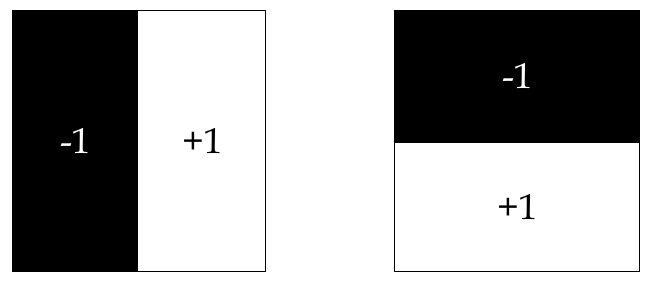
\includegraphics[width=0.75\textwidth]{fig/haarwavelet.png}
     \vspace{-1em}
    \begin{center}    
       \caption{\textcolor{gray}{\footnotesize \textit{ }}}
    \label{fig:haarwavelet}
     \end{center}
     \vspace{-2.5em}
  \end{figure} \noindent

SURF gør brug af Haar-wavelet, både i detektoren og deskriptoren. Haar-wavelet er et boks-filter, med størrelse nxn, hvor halvdelen af alle indgangene er +1 og den anden halvdel er -1.


\subsection{Deskriptor}
SURF deskriptoren producerer features, der består af 64 indgange. Den kan beskrives stringent, ligesom (26). Som beskrevet i SURF papiret af Tuytelaars et. al[??], er tilfældet ofte, at der ikke er brug for rotationsinvarians. En variant af SURF, der ikke er rotationsinvariant, kaldes Upright-SURF (U-SURF). Tuytelaars et. al garanterer dog rotationsinvarians i U-SURF, i op til $\pm 15^{\circ}$. SURF er implementeret, fremfor U-SURF, da enkelte af billederne har stor grad (ca. $15^{\circ}$) af rotation. Rotationen forekommer i billeder, der er taget lige efter, at dronen har vendt og kan ses på figur 15.
\\
\\
For at gøre SURF invariant overfor rotation, skal Haar-wavelet responset findes i x og y retningen omkring punktet ($dx, dy$), respektivt. $dx$ og $dy$ beregnes i en cirkel omkring interessepunktet, med radius $6\sigma$, og en afstand mellem punkterne, på $\sigma$. $dx$ og $dy$ foldes med en cirkulær Gausskerne, med samme størrelse som Haar-wavelet responsene, og $\sigma_{Gauss} = 2.5\sigma$.
\begin{figure}[H]
    \centering
    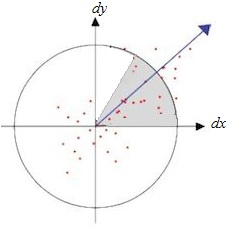
\includegraphics[width=0.2\textwidth]{fig/surforientation.jpg}
     \vspace{-1em}
    \begin{center}    
       \caption{\textcolor{gray}{\footnotesize \textit{ }}}
    \label{fig:surforientation}
     \end{center}
     \vspace{-2.5em}
  \end{figure} \noindent
Et sliding vindue på $60^{\circ}$, summerer alle vektorene, der ligger indenfor dets rækkevidde. Den længste vektor, udgør retningen, som beregnes med $atan2$ (invers tangens, med 2 inputs). Dette er illustreret på figur \ref{fig:surforientation}. Der er her taget en beslutning om, at slidingvinduet udregner summerne af vektorer, indenfor seks positioner ($0^{\circ}-60^{\circ}$, $60^{\circ}-120^{\circ}$.. $300^{\circ}-360^{\circ}$). 
\\
\\
SURF deskriptoren samler data omkring interssepunktet, med et dataindsamlingvindue der har størrelse $20 \sigma$. Vinduet skal orienters, ifht. den $\theta$ værdi, der er udregnet i detektoren. Billedet vendes, ved, at vende hele billedet, ved brug af ligning \eqref{rotaionmatrix}, og danne et integralbillede udfra det nye billede (Dette skridt er omkostningsfuldt, og der vil senere blive diskuteret optimeringer).
\\
\\
Dataindsamlingsvinduet er nu roteret og centreret omkring interessepunktet. Herefter skal vinduet deles op i 4x4 regioner, hver bestående af 5x5 punkter, der har ens afstand mellem sig - her er ikke blevet lavet subpixel-optimeringen, så hvis $\frac{20\sigma}{4}$ ikke er deleligt med 5, bliver der rundet ned.
\\
\\
Herefter skal Haar-wavelet responset udreges, i x og y retningen ($dx, dy$, respektivt). Haar-wavelet skal udregnes for alle punkter i 5x5 felterne. Størrelsen på Haar-wavelet filteret, er $2\sigma$. Disse værdier skal smoothes med et Gaussfilter, hvor $\sigma_{Gauss} = 3.3\sigma_{point}$.
\\
\\
For her af de 16 4x4 regioner, udregnes: 
\begin{equation}
v_i = \sum d_x, \sum d_y, \sum |d_y|, \sum |d_y|
\label{surffeature}
\end{equation}
hvor $v_i$ er beregningerne, for den $i$'ende region. Der laves en vektor, hvor alle værdierne indgange i $v$ sættes efter hinanden. Dette giver en $16 \cdot 4 = 64$ indgange stor vektor. Slutteligt, laves vektoren om til en enhedsvektor.

\subsubsection*{Algoritme}
\begin{enumerate}
\item Orienteringen findes: \begin{enumerate}

	\item Orienteringen på punktet findes, ved at beregne $dx$, $dy$ i et cirkulært område, med radius $6\sigma$, og afstand $\sigma$, mellem punkterne. 
	\item $dx$, $dy$ foldes med en Gauss kerne, med $\sigma_{Gauss} = 2.5\sigma $
	\item Den længste vektor, af summerede vektorer, der ligger indenfor $60^{\circ}$, bruges til at tildele orientering $\theta$ til interessepunktet.
\end{enumerate}
\item Et dataindsamlingsvindue roteret ifht. $\theta$, beregnet som \eqref{rotaionmatrix} med størrelse $20\sigma$ indsamler punkter, der er har afstand $\sigma$ mellem hinanden.
\item Haar-wavelet responset, $dx$, $dy$ udregnes for de indsamlede punkter, med en filterstørrelse på $2\sigma$, og $dx, dy$ foldes med Gauss, hvor $\sigma_{Gauss} = 3.3\sigma$
\item For hver af det 4x4 regioner, udregnes \eqref{surffeature}. Dette sættes sammen til en vektor, der vil have 64 indgange
\end{enumerate}